\chapter{Implementacja}
\label{cha:implementacja}
W ramach niniejszej pracy magisterskiej stworzono grę komputerową wykorzystującą przygotowywany prototyp interfejsu do  odczytu zmian stanów emocjonalnych i~zachowań gracza. Na podstawie analizy silników do tworzenia gier przeprowadzonej w~rozdziale~\ref{cha:specyfikacja} zdecydowano się na wykorzystanie platformy Unity. Głównym powodem takiej decyzji była przede wszystkim ilość materiałów o~tematyce tworzenia gier przy pomocy właśnie tego narzędzia, a~także dostępność rozwiązań, które pozwalały na prostą komunikację z~urządzeniami opisanymi w~rozdziale~\ref{cha:architektura}. 

\section{Podstawowe założenia}
Zanim rozpoczęto tworzenie gry, zostały określone założenia i~wymagania implementacyjne oraz projektowe, według których następnie został zbudowany projekt:
\begin{enumerate}
	\item Gra powinna zawierać mechaniki afektywne modyfikujące rozgrywkę w~zależności od zachowań lub stanu emocjonalnego gracza.
	\item Jednym z~elementów implementacyjnych powinien być interfejs umożliwiający komunikację z~urządzeniami opisanymi w~rozdziale~\ref{cha:architektura}. Moduł musi także komunikować się z~serwerem zawierającym model do predykcji emocji oraz w~prosty sposób udostępniać zmiany stanu emocjonalnego użytkownika i~jego zachowań. 
	\item Gra powinna mieć możliwość wyboru jednego z~dwóch trybów: podstawowego, zawierającego standardowe mechaniki gry, oraz wersję afektywną.
	\item Rozgrywka powinna być powtarzalna, aby w~trakcie przeprowadzania badań, każdy z~uczestników mógł doświadczyć tych samych elementów gry.
\end{enumerate}

\section{Implementacja gry}
%Opis gry, które elementy za co odpowiadają
Ponieważ przygotowywana gra miała być wykorzystana do przeprowadzenia eksperymentów w~celu ewaluacji opracowanego rozwiązania, zdecydowano się na grę jednoosobową. W~trakcie rozgrywki gracz wciela się w~rolę kapitana statku kosmicznego, który musi walczyć z~przeciwnikami, aby przeżyć. Jego zadaniem jest sterowanie pojazdem i~pokonanie jak największej liczby przeciwników przy pomocy dostępnego wyposażenia. Rozgrywka podzielona jest na poziomy, w~których trakcie gracz musi zdobyć określoną liczbę punktów. Na każdym z~poziomów dookoła statku generowanych jest kilka rodzajów wrogich statków. Schemat i~szybkość pojawiania się ich w~trakcie gry są zróżnicowane w~zależności od postępu. Z~każdym kolejnym poziomem pojawiają się nowe rodzaje jednostek, które mogą nie tylko lecieć w~kierunku w~gracza lub do niego strzelać pojedynczymi pociskami, ale również wybuchać w~jego pobliżu, posiadać większą wytrzymałość lub wykorzystywać inne rodzaje pocisków. Każdy z~przeciwników ma także przypisaną ilość punktów dodawaną do puli po zniszczeniu go. Aby przejść do kolejnego poziomu, gracz musi osiągnąć odpowiednio wysoki wynik.

Statek posiada ograniczoną liczbę punktów życia, która zwiększa się po przejściu każdego z~poziomów. Aby urozmaicić rozgrywkę, dookoła gracza mogą pojawić się także wzmocnienia w~postaci innych broni oraz obiektów leczących. Innym elementem mającym mocno wpłynąć na rozgrywkę jest moc specjalna umożliwiająca wypuszczenie fali w~kształcie okręgu, która natychmiastowo niszczy wrogie statki. Ponieważ umiejętność ta bardzo ułatwia rozgrywkę, gracz jest w~stanie użyć jej jedynie co określony czas. 

Aby wyrównać trudność gry i~nie znudzić graczy powtarzalną rozgrywką, każdy z~poziomów posiada także dodatkowy tryb charakteryzujący się zwiększeniem skomplikowania rozgrywki. Jest on uruchamiany na pewien określony czas po spełnieniu specjalnych warunków, które w~zależności od wersji gry są inne. W~trakcie trwania trybu trudnego schemat generowania przeciwników jest zmieniany na ich silniejsze wersje, posiadające większą ilość życia i~zmodyfikowane umiejętności. Podwojona zostaje także szybkość generowania przeciwników.

Cała gra została stworzona w~stylu dwuwymiarowym. Na rysunku~\ref{fig:ui} przedstawiony został fragment przykładowej rozgrywki. Oznaczone elementy interfejsu użytkownika to kolejno:
\begin{enumerate}
	\item \textbf{Pasek wskazujący poziom życia bohatera}. Warto zwrócić uwagę na brak oznaczenia dokładnej ilości punktów życia. Ukrycie tej informacji zmusza użytkownika do kontrolowania wartości tej cechy w~trakcie gry, a~także do unikania wszystkich przeciwników, niezależnie od tego, jakie obrażenia zadają.
	\item \textbf{Ikony aktualnie wybranej broni i~dostępności mocy specjalnej}. Służą one przede wszystkim jako elementy informacyjne. Wskazanie używanej broni pozwala graczowi na zorientowanie się, czy wzmocnienie w~postaci innego typu pocisków jest lepsze od aktualnie posiadanego. Ikona mocy specjalnej natomiast jest nie tylko wskazaniem jej dostępności. W~trakcie czasu pomiędzy kolejnymi jej użyciami ikona ta spełnia funkcję orientacyjnego licznika, który wskazuje użytkownikowi, kiedy ponownie będzie mógł z~niej skorzystać.
	\item \textbf{Ilość punktów zdobytych przez gracza oraz pasek postępu dla danego poziomu}. Podobnie jak w~przypadku ilości życia, pokazywany jest jedynie orientacyjny postęp gracza na danym poziomie, dzięki czemu użytkownik nie jest do końca pewien, kiedy ukończy poziom. Z~drugiej strony wyświetlana jest suma punktów zdobytych w~trakcie całej rozgrywki, co stanowi pewnego rodzaju motywację dla gracza, aby zdobyć jak najwyższy wynik.
\end{enumerate}

\begin{figure}
	\centering
	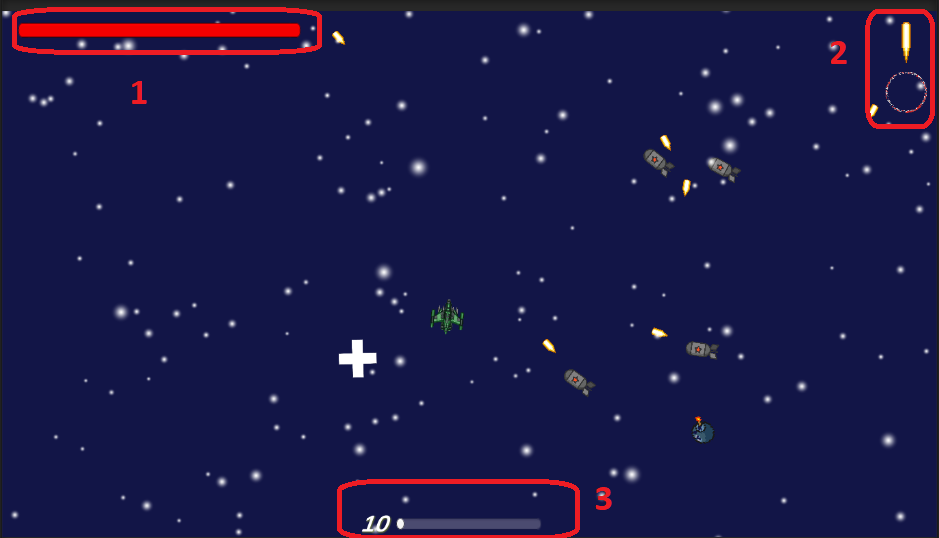
\includegraphics[width=0.7\linewidth]{images/ui.png}
	\caption{Ekran gry z~oznaczonymi elementami interfejsu użytkownika}
	\label{fig:ui}
\end{figure}

Tak jak zostało wspomniane na początku rozdziału, do implementacji gry wykorzystano silnik Unity. W~momencie tworzenia projektu zdecydowano się na użycie wersji 2018.3.0f2 przeznaczonej do budowania gier na systemy operacyjne oparte o~architekturę 64-bitową. Ponieważ projektowanie gier przy pomocy tego silnika polega na tworzeniu elementów, które są wprowadzane w~interakcje pomiędzy sobą, a~logika za to odpowiadająca zawarta jest w~skryptach dołączanych do obiektów, zdecydowano się na stworzenie hierarchii, gdzie pierwszym poziomem są poszczególne elementy rozgrywki umieszczane na scenie gry, drugim natomiast są skrypty odpowiadające za logikę danego obiektu lub innych elementów takich jak interfejs użytkownika czy postępy gracza. Do obiektów stanowiących główne elementy świata gry należą:
\begin{enumerate}
	\item \textbf{Player} reprezentujący statek, którym kieruje gracz. Poza elementami graficznymi zawiera on następujące skrypty związane ze sterowanym statkiem:
	\begin{itemize}
		\item \textbf{PlayerController}, opisujący sposób poruszania się kontrolowanego statku. Przy jego pomocy ustawiana są także prędkość oraz czas potrzebny na wyhamowanie pojazdu.
		\item \textbf{PlayerShooter}, odpowiadający za logikę strzelania wybraną bronią, a~także za użycie mocy specjalnej. Jej głównym zadaniem jest zarządzanie tworzeniem pocisków i~aktywacji animacji oraz dźwięków związanych ze strzałem lub aktywacją mocy specjalnej. Skrypt odpowiada także za integrację z~elementami interfejsu użytkownika odpowiedzialnymi za wyświetlanie aktualnie używanej broni i~dostępności mocy specjalnej. Umożliwia on także zmianę wykorzystywanej broni oraz zarządzanie parametrem czasu odnowienia mocy specjalnej. 
		\item \textbf{Player}, odpowiadający za kontrolowanie życia postaci. Mowa tutaj nie tylko o~zmniejszaniu jego ilości po przyjęciu obrażeń lub zwiększaniu podczas leczenia bohatera, ale również ustawianiu nowej wartości maksymalnej punktów życia po zakończeniu poziomu. Skrypt ten zarządza elementem interfejsu użytkownika odpowiedzialnym za wyświetlanie aktualnej ilości życia. Kontroluje także wywołanie animacji i~dźwięków uruchamianych po śmierci bohatera, a~także oddelegowanie akcji odpowiedzialnych za zatrzymanie gry do obiektów sterujących rozgrywką.
	\end{itemize}

	\item \textbf{Obiekty reprezentujące przeciwników}. Każdy z~nich różnił się przypisanymi elementami graficznymi oraz skryptami, które mogą różnić się w~zależności od typu przeciwnika. Do skryptów sterujących logiką przeciwników należą:
	\begin{itemize}
		\item \textbf{Enemy}, odpowiadający przede wszystkim za zarządzanie poziomem życia przeciwnika, zmniejszaniu go po zadaniu obrażeń przez gracza, zmianie elementów graficznych w~zależności od ilości punktów życia przeciwnika, oraz za wywołanie animacji i~dźwięków mających nastąpić po śmierci przeciwnika. Skrypt posiada także parametr związany z~ilością obrażeń zadawanych podczas zderzenia z~graczem i~zarządza samą akcją kolizji, zabierając graczowi ustaloną ilość punktów życia.
		\item \textbf{EnemyMovement}, odpowiadający za sposób poruszania się przeciwnika. W~zależności od typu wroga, skrypt zarządza czy ma się on zbliżać do gracza, okrążać go, czy może stać w~miejscu. Zawiera on parametry dotyczące szybkości przeciwnika, maksymalnej odległości od gracza, oraz dystansu od niego, na jakim część przeciwników ma się zatrzymać.
		\item \textbf{EnemyShooter}, odpowiadający za kontrolę strzałów przeciwnika, ich szybkość, stworzenie pocisków oraz wywołanie efektów dźwiękowych strzału. Skrypt ten jest przypisywany wyłącznie do przeciwników typu strzelającego.
		\item \textbf{EnemyBomber}, zarządzający logiką wybuchu przeciwnika. Kontroluje przede wszystkim zadanie graczowi obrażeń i~odepchnięcie innych przeciwników, jeśli znajdują się w~zadanej przez parametr odległości. Odpowiada także za uruchomienie animacji oraz dźwięku związanych z~odliczaniem do wybuchu.
	\end{itemize}
	
	\item \textbf{Obiekty reprezentujące wzmocnienia, które gracz może zdobyć w~trakcie rozgrywki}. Poza elementami graficznymi, w~zależności od rodzaju ulepszenia, każdy z~nich ma przypisany do siebie następujące skrypty:
	\begin{itemize}
		\item \textbf{PowerUp}, odpowiadający za wywołanie efektu wzmacniającego gracza, oraz ciągły obrót obiektu wzmocnienia. Jest to skrypt abstrakcyjny, co oznacza, że nie jest przypisany bezpośrednio do elementu, a~stanowi bazę dla skryptów mogących rozszerzać jego zachowanie. W~tym przypadku rozszerzeniem jest funkcja odpowiedzialna za nałożenie efektu wzmacniającego na gracza.
		\item \textbf{HealthPowerUp}, będący rozszerzeniem skryptu PowerUp. W~ramach wzmocnienia skrypt przywracał pewną ilość punktów życia określoną przez parametr.
		\item \textbf{WeaponPowerUp}, będący rozszerzeniem skryptu PowerUp. Wzmocnienie w~tym przypadku polegało na zmianie broni gracza na tę, która była przypisana do wzmocnienia w~formie parametru.
	\end{itemize}
\end{enumerate}

Poza wyżej wymienionymi elementami, stanowiącymi część gry widoczną dla gracza, stworzone zostały obiekty będące częścią menu głównego, a~także nieposiadające reprezentacji graficznej elementy zarządzające. Do każdego z~nich został przypisany skrypt odpowiadający za kontrolowanie innych elementów rozgrywki:
\begin{itemize}
	\item \textbf{MainMenu}, zawierający metody uruchamiające oraz zamykające grę. W~ramach funkcji inicjującej rozgrywkę skrypt uruchamiał animacje wyświetlające ekran powitalny, a~następnie rozpoczynał faktyczną rozgrywkę.
	\item \textbf{PowerUpGenerator}, odpowiadający za generowanie obiektów wzmocnień w~trakcie gry. Kontrolował on tworzenie wybranego ulepszenia w~losowo wybranej pozycji w~określonej odległości od gracza. Ilość wzmocnień znajdujących się  w~trakcie gry jest ograniczona, aby użytkownik odczuł, że są to elementy wyjątkowe. Wartość ta, wraz z~częstotliwością generowania wzmocnień i~odległością od gracza, w~jakiej obiekty mają być generowane, sterowane są przez parametry skryptu. 
	\item \textbf{EnemySpawner}, wykorzystywany do zarządzania logiką odpowiadającą za generowanie przeciwników w~świecie gry. Skrypt ten posiadając określoną w~parametrze listę szablonów wrogich jednostek, które mają być generowane, co pewien czas tworzy każdego z~przeciwników w~formie fali. Każdy z~nich pojawia się w~losowo dobranych miejscach. Częstotliwość fal i~odległość, w~jakiej przeciwnicy są generowani od gracza, określane są poprzez parametry skryptu.
	\item \textbf{GameManager}, zarządzający zatrzymywaniem rozgrywki, oraz sterowaniem elementami po zakończeniu gry. Skrypt ten kontrolował flagi blokujące wszystkie inne obiekty w~przypadku zatrzymania gry. Odpowiadał on także za wywołanie animacji wyświetlanych po śmierci gracza, zmianę sceny podczas wyjścia z~gry, czy jej ponowne uruchomienie w~przypadku chęci ponownego rozpoczęcia rozgrywki.
	\item \textbf{Progress}, będący miejscem sterującym postępami gracza. Przy jego pomocy gromadzone są punkty zdobyte w~trakcie rozgrywki. Po zdobyciu punktów skrypt sprawdza, czy przekroczony został wynik wymagany do ukończenia poziomu. Jeżeli tak to  ze sceny usuwane są wszystkie obiekty przeciwników i~pociski, a~następnie w~zależności od tego, czy dany poziom był ostatni, uruchamia funkcje odpowiadające za zakończenie gry lub przejście do kolejnego poziomu. W~przypadku końca rozgrywki, skrypt aktywuje animację wyświetlającą gratulacje dla gracza, a~następnie oznacza rozgrywkę jako zakończoną przy pomocy flagi ze skryptu GameManager. W~przypadku przejścia na kolejny poziom aplikowana jest nagroda w~postaci zwiększonych punktów życia, a~następnie ładowane są parametry nowego poziomu. Jednocześnie, niezależnie od tego, czy gracz ukończył poziom, aktualizowane są elementy interfejsu wyświetlającego ilość zdobytych punktów oraz sprawdzany jest warunek wymagany do uruchomienia trybu trudnego gry. Jeżeli został on spełniony, to lista generowanych przeciwników zostaje zmieniona na trudniejszą wersję, a~częstotliwość fal jest podwajana. W~ramach parametrów skryptu należy wyróżnić warunki uruchomienia trybu trudnego i~czas jego trwania, a~także listę poziomów w~grze. Ten ostatni parametr stanowi główny rdzeń rozgrywki, ponieważ zawiera w~sobie szablon każdego z~poziomów, na który składają się: listy generowanych przeciwników, zarówno w~wersji klasycznej, jak i~trudnej, częstotliwość fal wrogów, wynik wymagany do ukończenia poziomu, liczba punktów życia dodana graczowi po jego ukończeniu, a~także flaga oznaczająca czy dany poziom jest ostatnim.
\end{itemize}

Wszystkie powyższe elementy stanowiły bazę dla podstawowej wersji gry. Parametry każdego z~obiektów zostały dobrane tak, aby gracz odczuwał postęp, który ma doprowadzić go ostatecznie do końca gry. Struktura projektu została zachowana w~formie dwóch scen, jednej odpowiedzialnej za menu gry, w~drugiej natomiast odbywała się faktyczna rozgrywka. Tak jak to zaznaczono podczas opisywania skryptów, całość gry odbywa się w~jednej scenie. Wynika to przede wszystkim z~powtarzalności poziomów różniących się między sobą wyłącznie parametrami. 

Ostatnim etapem tworzenia podstawowej wersji gry było dostosowanie sterowania do wykorzystywanego kontrolera Dualshock 4. Ponieważ Unity dla każdej z~gier może mieć zdefiniowaną listę nazw odpowiadającym danym przyciskom lub elementom, które mają pewien zakres działania, poza przystosowaniem standardowych nazw do odpowiednich przycisków na kontrolerze, dodane zostały osie zawierające w~sobie odczyty z~prawego analoga kontrolera. Pozwoliło to na wykorzystanie go do kontrolowania kierunku, w~którym miał się obracać statek.

\section{Odczyt danych fizjologicznych i~zmian emocji}
%Opis elementów do odczytu emocji i~EMG, odczyty z~cheststrapa, komunikacja z~serwerem
Równolegle, w~trakcie tworzenia implementacji podstawowej gry, stworzony został moduł umożliwiający pobieranie danych fizjologicznych i~odczytów akcelerometru z~urządzeń opisanych w~rozdziale~\ref{cha:architektura}. Pobrane informacje wykorzystano do przygotowania prostego interfejsu umożliwiającego implementację mechanizmów oddziaływania na strukturę gry w~zależności od otrzymanych danych i~tym samym domknięcie pętli afektywnej.

Pierwszym krokiem było przygotowanie skryptów umożliwiających odczyt sygnałów bezpośrednio z~urządzeń. W~przypadku BITalino (r)evolution kit skorzystano z~rozwiązania dostępnego na stronie producenta~\cite{bitalino_apis}. Aby uniknąć ewentualnych problemów z~kompatybilnością, spośród dostępnych interfejsów programistycznych na platformę Unity, wybrano ten dostosowany do wyższych wersji oprogramowania. Bazując na przykładach oferowanych w~ramach interfejsu, stworzony został obiekt BITalino, który w~pełni będzie odpowiadał za integrację z~urządzeniem. Przypisano do niego następujące skrypty:
\begin{itemize}
	\item \textbf{BitalinoSerialPort}, udostępniony jako część wykorzystanego interfejsu. Skrypt umożliwiał konfigurację parametrów związanych z~nawiązaniem połączenia z~płytką poprzez transmisję szeregową, zarówno przez Bluetooth, jak i~kabel USB. W~ramach parametrów możliwe było ustawienie między innymi limitów czasu oczekiwania na odczyt i~zapis danych, jednak najistotniejsza była możliwość wprowadzenia nazwy kanału, przy pomocy którego możliwa była komunikacja z~urządzeniem. 
	\item \textbf{BitalinoManager}, udostępniony jako część wykorzystanego interfejsu. Skrypt ten umożliwia przede wszystkim konfigurację listy wykorzystywanych kanałów i~określenia, jakiego rodzaju sygnały są przypisane do każdego z~nich. W~przypadku przygotowywanego projektu ustalony został wyłącznie jeden kanał przyjmujący odczyty z~elektromiogramu. Skrypt umożliwia także ustalenie częstotliwości wysyłania danych. Ze względu na chęć uzyskania jak najdokładniejszych pomiarów, zdecydowano się na ustawienie najwyższej możliwej wartości, czyli tysiąca próbek na sekundę.
	\item \textbf{BitalinoReader}, udostępniony jako część wykorzystanego interfejsu. Skrypt służy do zarządzania przetwarzaniem danych z~płytki, tego, w~jakiej postaci są one zwracane, oraz jak wielki jest bufor, w~którym są przechowywane. Jego rozmiar ustawiono na sto ostatnich elementów. Wybór takiej wartości wynika przede wszystkim ze względu na chęć uzyskania jak najmniejszego opóźnienia od momentu otrzymania pomiarów bezpośrednio z~urządzenia do czasu wykorzystania ich przetworzonej wersji. Ponieważ sygnał z~elektromiografu ma służyć wykryciu zmian w~napięciu mięśni, nie była tutaj wymagana wysoka ilość próbek.
	\item \textbf{SensorController}, przygotowany w~ramach niniejszej pracy magisterskiej. Głównym zadaniem tego skryptu był odczyt w~czasie rzeczywistym bufora danych, wyznaczanie średniej z~wartości bezwzględnych pomiarów z~elektromiografu, a~następnie sprawdzenie, czy przez określony czas miało miejsce napięcie mięśni przedramienia. Użycie wartości bezwzględnej wynika z~oscylacji występujących w~sygnale pobranym z~elektromiografu. Wykrycie napięcia zostało oparte na warunku:
	$$
	|EMG|_{avg} \geq mul \cdot |EMG|_{base}
	$$
	gdzie $|EMG|_{avg}$ jest aktualnie odczytaną średnią wartością, $mul$ mnożnikiem ustawianym jako parametr umożliwiający regulację wykrycia napięcia mięśni, a~$|EMG|_{base}$ średnim pomiarem bazowym. Ostatnia z~wartości jest wyznaczana podczas fazy kalibracji odbywającej się po rozpoczęciu pomiarów. Przez ustaloną parametrem ilość sekund, w~których trakcie użytkownik nie powinien napinać mięśni przedramienia, zbierane są odczyty z~elektromiografu, a~następnie na ich podstawie obliczana jest wartość służąca jako pomiar referencyjny, z~którym porównywane są odczyty w~trakcie rozgrywki.
\end{itemize}
Dodanie czasu, przez jaki miał być napięty mięsień oraz mnożnika w~warunku miało na celu odrzucenie krótkich, losowych ruchów ręką, jakie mogły wystąpić w~trakcie korzystania z~kontrolera. Pozwoliło to także dać użytkownikowi świadomość kontroli nad napięciem mięśni, ponieważ musiał wykonać tę czynność przez określony czas.

Aby obiekty, mające reagować na napięcie mięśni, mogły w~prosty sposób być o~tym informowane, został wykorzystany mechanizm zdarzeń z~języka C\#. W~ramach skryptu SensorController przygotowano delegata, będącego typem przechowującym referencję do metody i~określającym jakie parametry i~typ zwrotny powinna zawierać metoda, której sygnaturę określa delegat. Następnie dodane zostało zdarzenie o~typie przygotowanego delegata służące jako miejsce rejestracji i~wywołania metod, które mają obsłużyć daną sytuację. W~przypadku skryptu SensorController jest ono wywoływane w~momencie wykrycia napięcia mięśni przez określony czas. Tak przygotowany mechanizm pozwala na prawie całkowite uniezależnienie elementów związanych z~pomiarami fizjologicznymi od skryptów będących częścią implementacji gry.

Kolejnym krokiem było przygotowanie skryptów do odczytu sygnałów z~opaski Garmin HRM-Run i~akcelerometru wbudowanego w~kontroler Dualshock. Zostaną one następnie wykorzystane w~skryptach komunikujących się z~modelem opisanym rozdziale~\ref{cha:predykcja} i~zwracających odczyty emocji odczuwanych przez użytkownika w~trakcie rozgrywki.

Podobnie jak w~przypadku odczytów z~płytki BITalino (r)evolution kit, do pomiaru tętna wykorzystana została biblioteka do obsługi protokołu ANT+ oraz przykład znajdujące się na stronie producenta~\cite{ant_sdk}. Przy ich pomocy przygotowano następujące skrypty umożliwiające pomiar tętna z~opaski:
\begin{itemize}
	\item \textbf{AntReader}, przygotowany na podstawie przykładu udostępnionego przez twórców biblioteki. Kod został dostosowany w~taki sposób, aby można było uruchomić odczyt przy pomocy funkcji. Do najważniejszych parametrów skryptu należy przede wszystkim numer i~typ urządzenia, z~jakiego mają być odbierane dane. Ponieważ odczyty z~czujnika przychodzą w~formie ramki z~danymi, do skryptu dodany został parser tworzący obiekt zawierający informacje na temat wartości tętna, ilości uderzeń od rozpoczęcia pomiarów, czas ostatniego odczytu, oraz wartość interwału pomiędzy ostatnimi dwoma uderzeniami w~milisekundach. Tak przygotowany obiekt jest następnie wysyłany jako parametr zdarzenia, które także zostało dodane jako modyfikacja przykładu. Takie podejście wynika przede wszystkim z~protokołu bazującego na przesyłaniu zdarzeń w~momencie wystąpienia akcji.
	\item \textbf{HeartRateManager}, zarządzający danymi przesyłanymi przez skrypt AntReader. Jego głównym zadaniem jest przechowywanie obiektów z~informacją na temat pracy serca w~buforze, którego rozmiar jest zadany przez parametr. Skrypt ten umożliwia także wyizolowanie z~bufora wartości tętna i~interwałów pomiędzy uderzeniami w~formie tablic.
\end{itemize}

W przypadku odczytów akcelerometru z~kontrolera Dualshock 4~producent udostępnia oprogramowanie wbudowane w~silnik Unity, jednak jest ono dostępne wyłącznie dla osób projektujących gry na konsolę PlayStation 4. W~związku z~tym wykorzystany został odpłatny dodatek Rewired, udostępniający obsługę wielu kontrolerów do gier, nie tylko na poziomie obsługi przycisków, ale również wbudowanych funkcjonalności takich jak kontrola wibracji, oświetlenia, czy odczytów z~sensorów zawartych w~kontrolerze, do których można zaliczyć akcelerometr oraz żyroskop. Do odbierania sygnałów z~kontrolera i~ich interpretacji przygotowane zostały następujące skrypty:
\begin{itemize}
	\item \textbf{AccelerationReader}, odpowiadający za pomiar i~wstępną filtrację danych z~akcelerometru. Częstotliwość odczytu jest ustalana za pomocą parametru skryptu, a~każda odebrana wartość jest filtrowana przy pomocy filtru Kalmana, aby pozbyć się ewentualnych szumów.
	\item \textbf{AccelerationHandler}, odpowiadający za przechowywanie i~analizę pomiarów odebranych przez skrypt AccelerationReader. Dane przechowywane są w~dwóch listach: jednej przeznaczonej do fazy kalibracji oraz drugiej będącej buforem odczytów z~określonej parametrem ilości czasu. Do wyznaczenia aktywności użytkownika wykorzystano zryw, czyli zmianę wartości przyspieszenia w~czasie. Podczas fazy kalibracji po zebraniu danych z~akcelerometru do przygotowanej listy obliczana była średnia wartość zrywu, która posłuży jako pomiar referencyjny. W~ramach jednej z~funkcji skrypt umożliwia pobranie aktualnej aktywności użytkownika w~postaci jednego z~trzech stanów: bardzo spokojny, spokojny i~podekscytowany. Funkcja oblicza wartość zrywu z~aktualnie zapisanych pomiarów, a~następnie określa czy użytkownik jest podekscytowany na podstawie warunku:
	$$
	jerk_{avg} \geq mul \cdot jerk_{base}
	$$
	gdzie $jerk_{avg}$ jest aktualnie odczytaną wartością zrywu, $mul$ mnożnikiem ustawianym jako parametr umożliwiający regulację poziomu granicznego dla ekscytacji, a~$jerk_{base}$ jest pomiarem zrywu uzyskanym w~trakcie kalibracji. Następnie, jeśli stan nie został określony jako ekscytacja, sprawdzana jest ostatnio odczytana wartość aktywności użytkownika. Jeżeli gracz był spokojny, a~ostatni pomiar odbył się w~określonym czasie, to skrypt uznawał gracza za bardzo spokojnego. W~przeciwnym wypadku zwracany był stan spokojny.
\end{itemize}

Tak przygotowane skrypty do odczytu i~wstępnej analizy danych z~czujnika do pomiaru tętna i~akcelerometru zostały następnie wykorzystane do ustalenia stanu emocjonalnego użytkownika. Umieszczono je w~obiekcie EmotionManager, który skupia wszystkie skrypty odpowiedzialne za określenie emocji gracza. Aby powiązać odczytane dane z~modelem uczenia maszynowego oraz wyznaczyć odczuwane przez użytkownika emocje, do obiektu EmotionManager dodane zostały następujące skrypty:
\begin{itemize}
	\item \textbf{ClassifierApiManager}, odpowiadający za komunikację z~serwerem zawierającym model rozpoznający emocje. Skrypt wykorzystując dane na temat tętna i~interwałów pomiędzy kolejnymi uderzeniami znajdujące się w~skrypcie HeartRateManager, wykonuje zapytanie HTTP do serwera i~zapisuje zwracana klasę emocji oraz parametry, dla których dana wartość została zwrócona. Skrypt zawiera także flagę informującą, czy od momentu ostatniego odczytu emocji przez inne skrypty była ona aktualizowana.
	\item \textbf{EmotionManager}, zarządzający pozostałymi skryptami do wyznaczania stanu emocjonalnego, a~także będący punktem wyjściowym dla przekazywania go do innych obiektów. Głównym zadaniem skryptu jest uruchomienie pobierania danych z~opaski i~akcelerometru, a~następnie określenie emocji użytkownika na podstawie klasy zwróconej przez model rozpoznający emocję oraz stanu pobudzenia zwracanego przez skrypt AccelerationHandler. W~momencie pobierania emocji wywoływane jest zapytanie do serwera przy pomocy skryptu ClassifierApiManager o~stan emocjonalny użytkownika na podstawie danych z~opaski. Zwrócona klasa emocji jest konwertowana do obiektu zawierającego poziomy wartości \textit{valence} i~\textit{arousal}, a~następnie przy pomocy odczytanego z~akcelerometru stanu pobudzenia, są one weryfikowane. Ponieważ pomiar \textit{arousal} jest związany bezpośrednio z~pobudzeniem gracza, to właśnie ta wartość była modyfikowana. Jeżeli stan zwracany przez odczyty z~akcelerometru wskazywał na pobudzenie użytkownika, poziom \textit{arousal} zostaje zwiększony, natomiast w~przypadku bardzo spokojnej gry, jest on zmniejszany. Dzięki takiemu podejściu można łatwo weryfikować klasę zwracaną przez model, która nie zawsze mogła dokładnie odzwierciedlać stan emocjonalny gracza w~danym momencie rozgrywki. Po odczytaniu stanu emocjonalnego następowało wywołanie zdarzenia o~nowej emocji, które jako parametry przyjmowało wartość odczytaną w~danym momencie oraz stan poprzedni. Wykorzystanie poprzednio odczytanego stanu miało na celu rozszerzenie kontekstu zmian emocji użytkownika i~ich interpretację przez konkretne elementy gry. Do najważniejszych parametrów skryptu EmotionManager należą przede wszystkim czas poświęcony na kalibrację oraz parametr określający co ile ma zostać wykonane zapytanie o~stan emocjonalny użytkownika. 
\end{itemize}

Obiekty BITalino i~EmotionManager zostały następnie połączone w~hierarchii pod obiektem AffectiveManager. Można traktować go jako rdzeń przygotowywanego w~ramach pracy magisterskiej interfejsu. Tak przygotowana hierarchia umożliwiała łatwe jego wprowadzenie do istniejącego już kodu gry. Do obiektu AffectiveManager został przypisany także skrypt o~tej samej nazwie, którego głównymi zadaniami było uruchamianie oraz wyłączanie mechanizmów opisanych powyżej, a~także rozpoczynanie fazy kalibracji dla pomiarów z~akcelerometru oraz odczytów z~elektromiografu. Dodany został także obiekt Logger odpowiadający za zapisywanie informacji o~odczuwanych stanach emocjonalnych oraz momentach wykrycia napięcia mięśni. W~przypadku odczytywania emocji zapisywane są poziomy \textit{valence} i~\textit{arousal} po weryfikacji pomiarami z~akcelerometru oraz wartości cech, dla których zostały one wyliczone. Pomiary te mogą posłużyć jako dodatkowe dane uczące mogące poprawić skuteczność modelu opisanego w~rozdziale~\ref{cha:predykcja}. W~przypadku odczytów z~elektromiografu zapisywane są momenty napięcia mięśni przedramienia wraz ze średnią wartością z~elektromiografu. Każde zdarzenie jest przechowywane w~pamięci wraz z~czasem jego wystąpienia, a~w momencie zakończenia rozgrywki są one zapisywane do pliku.

\section{Domknięcie pętli afektywnej}
Po stworzeniu opisanego w~poprzedniej sekcji interfejsu kolejnym krokiem było domknięcie pętli afektywnej. Oznaczało to uzależnienie pewnych elementów gry od stanu emocjonalnego i~reakcji użytkownika. Aby to osiągnąć, wymagana była modyfikacja podstawowej wersji gry i~zmiana działania jej mechanik w~zależności od wartości zwracanych przez skrypty EmotionManager i~SensorController.

Aby umożliwić integrację gry z~interfejsem, w~głównym menu gry przygotowana została opcja, która decyduje o~tym, czy mechaniki afektywne mają zostać uruchomione po rozpoczęciu gry. Następnie, w~ramach skryptu MainMenu, zmodyfikowany został proces wyświetlania wprowadzenia. W~przypadku wersji afektywnej wyświetlony zostaje tekst informujący użytkownika o~przeprowadzanej na początku kalibracji interfejsu oraz zasadach, których powinien przestrzegać w~trakcie jej trwania (rys.~\ref{fig:introductions}). Użytkownik proszony jest o~uspokojenie się, wzięcie kilku głębokich oddechów oraz nieporuszanie kontrolerem w~trakcie przeprowadzania kalibracji. W~tym samym momencie uruchamiany zostaje odczyt danych z~urządzeń pomiarowych, a~po kilku sekundach rozpoczynana jest kalibracja trwająca przez określony w~parametrach interfejsu czas. Wcześniejsze uruchomienie odczytu pozwoliło na odrzucenie pierwszych pomiarów z~urządzeń, które mogły charakteryzować się dużym błędem ze względu na start sprzętu.
\begin{figure}
	\begin{subfigure}{0.5\textwidth}
		\centering
		
\includegraphics[width=0.9\linewidth]{images/nonaffectiveintroduction.png}
		\caption{Wprowadzenie w~wersji podstawowej}
		\label{fig:nonaffectiveintroduction}
	\end{subfigure}%
	\begin{subfigure}{0.5\textwidth}
		\centering
		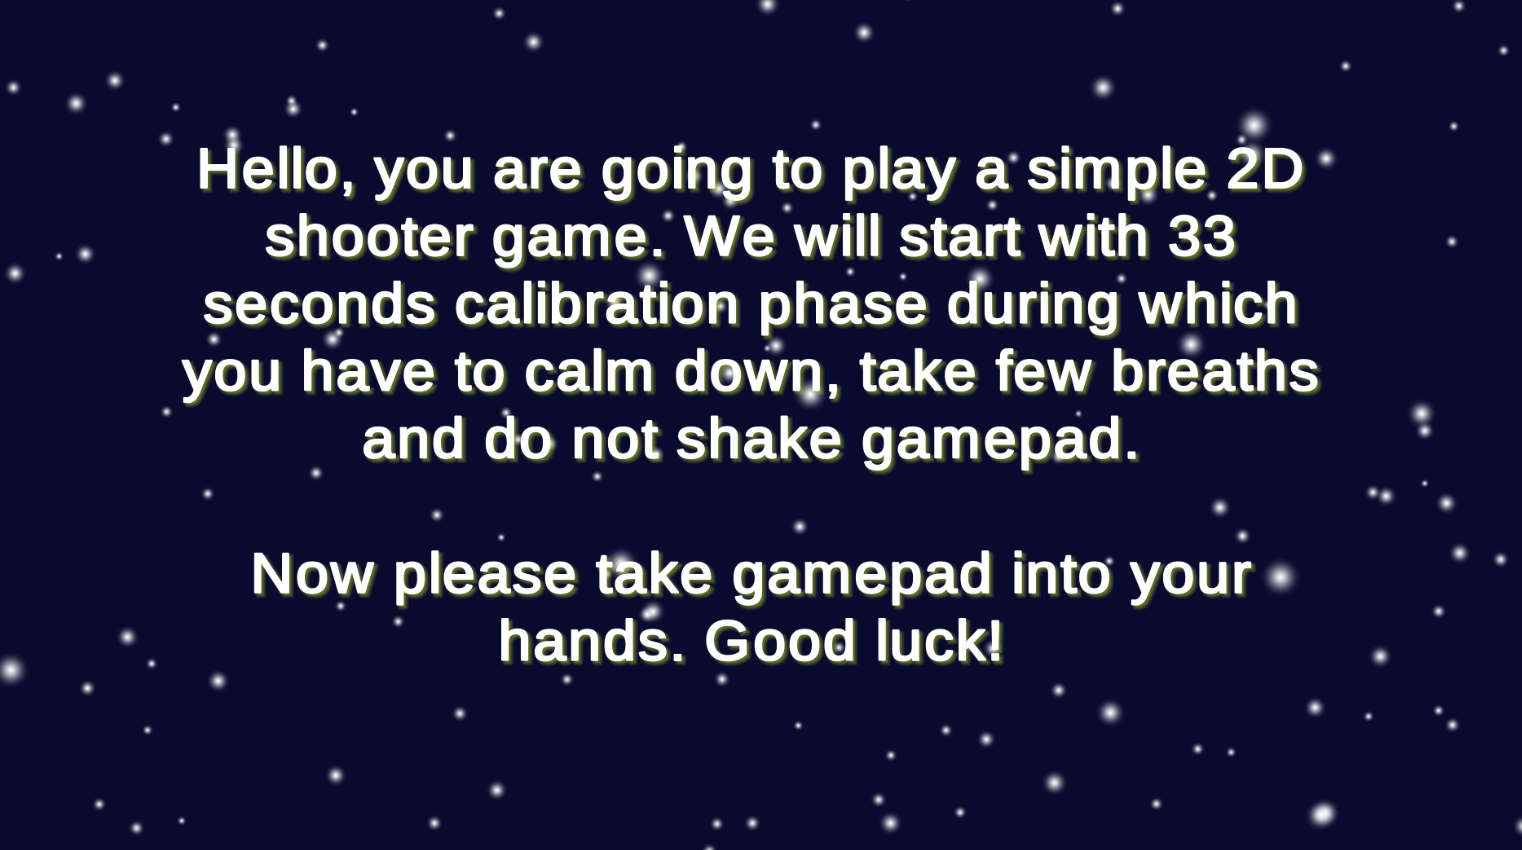
\includegraphics[width=0.9\linewidth]{images/affectiveintroduction.png}
		\caption{Wprowadzenie w~wersji afektywnej}
		\label{fig:affectiveintroduction}
	\end{subfigure}
	\caption{Ekran wprowadzenia dla obu wersji gier}
	\label{fig:introductions}
\end{figure}

Kolejnym krokiem w~integracji interfejsu było przygotowanie mechanik afektywnych, które wpływają na poszczególne elementy rozgrywki w~zależności od odczuwanych przez użytkownika emocji lub napięcia mięśni przedramienia. W~ramach skryptów odpowiadających za konkretne elementy rozgrywki przygotowane zostały funkcje, które następnie zarejestrowano jako obserwatorów wystąpienia nowej emocji lub napięcia mięśni. Aby ułatwić interpretację poziomów \textit{valence} i~\textit{arousal} zwracanych w~ramach obiektu reprezentującego odczuwaną emocję, stworzone zostały stałe, które przypisują każdą z~par obu wartości do konkretnej emocji. Interpretacja każdej z~kombinacji została przedstawiona w~tabeli~\ref{tab:emotions}. W~ramach zaimplementowanych mechanik afektywnych można wyróżnić:
\begin{enumerate}
	\item \textbf{Aktywacja mocy specjalnej po wykryciu napięcia mięśni przedramienia}. Mechanika ta stanowi alternatywę dla uruchomienia tej mechaniki przy pomocy przycisku na kontrolerze. Uruchomienie jej bez wyłączania akcji z~podstawowej wersji gry pozwala użytkownikowi wybrać sposób aktywacji, który jest dla niego wygodniejszy.
	\item \textbf{Aktywacja mocy specjalnej w~momencie, gdy gracz przez dłuższy czas odczuwa złość}. W~odróżnieniu od poprzedniego punktu, w~tym przypadku moc specjalna aktywowana jest niezależnie od jej dostępności w~momencie, gdy poprzednia i~aktualnie odczytana emocja to złość. 
	\item \textbf{Zmiana ilości punktów życia gracza na podstawie odczuwanych emocji}. Można wyróżnić tutaj następujące możliwości:
	\begin{itemize}
		\item Odebranie graczowi 40\% punktów życia w~przypadku odczuwania przez dłuższy czas emocji neutralnej, zmęczenia lub zrelaksowania. Taka reakcja miała na celu pobudzenie gracza do skupienia się na rozgrywce ze względu na nagłą trudną sytuację.
		\item Odebranie graczowi 20\% punktów życia w~momencie odczuwania przez dłuższy czas szczęścia lub ekscytacji. Emocje te zostały wydzielone do lżejszej wersji negatywnego efektu, aby uniknąć nadmiernego zdenerwowania gracza, ale jednocześnie wzbudzić w~nim potrzebę skupienia się na grze.
		\item Przywrócenie 10\% punktów życia w~momencie odczuwania smutku lub strachu. Efekt ten miał posłużyć jako pomoc dla gracza i~wywołanie przez to u niego pozytywnych emocji.
	\end{itemize}
	\item \textbf{Aktywacja dodatkowych fal przeciwników w~momencie odczuwania emocji neutralnej, zrelaksowania, zmęczenia lub szczęścia}. W~przypadku trzech pierwszych stanów emocjonalnych mechanika ta miała na celu postawienie graczowi wyzwania. Uruchomienie jej w~momencie odczuwania szczęścia przez gracza miało na celu wywołanie u niego emocji przeciwstawnych takich jak strach czy złość.
	\item \textbf{Aktywacja i~dezaktywacja trybu trudnego gry w~zależności od odczuwanej emocji}. Mechanika ta zastępowała jej podstawową wersję opartą na częstotliwości zdobywania punktów. W~przypadku odczuwania przez użytkownika złości lub strachu była ona dezaktywowana, natomiast aktywacja następowała w~momencie doświadczania przez gracza emocji neutralnej, zrelaksowania lub zmęczenia.
\end{enumerate}

\begin{table}
	\centering
	\caption{Interpretacja kombinacji poziomów \textit{valence} i~\textit{arousal} jako emocje.}
	\label{tab:emotions}
	\begin{tabular}{|l|l|l|l|}
		\hline
		\diagbox[width=8em]{\textbf{Valence}}{\textbf{Arousal}}      & LOW    & MEDIUM           & HIGH          \\ \hline
		LOW    & Smutek & Złość        & Strach \\ \hline
		MEDIUM & Zmęczenie  & Emocja neutralna & Zaskoczenie     \\ \hline
		HIGH   & Zrelaksowanie & Szczęście      & Ekscytacja    \\ \hline
	\end{tabular}
\end{table}

Implementacja interfejsu do rozpoznawania emocji i~zachowań gracza umożliwiła stworzenie gry zawierającej pętlę afektywną. Aby zrealizować w~pełni założenia programowania afektywnego, każda z~mechanik zmieniała rozgrywkę w~taki sposób, aby wzbudzić w~użytkowniku inny rodzaj emocji od aktualnie odczuwanych. Przygotowany interfejs umożliwił łatwą implementację każdej z~nich bez konieczności modyfikacji oryginalnego kodu gry dzięki rejestracji funkcji uruchamianych w~momencie odczytania emocji.
